% !TEX root = ../thesis.tex
%
\chapter{Einleitung}
\label{sec:intro}
Wikipedia ist die bekannteste freie Wissenssammlung im Internet.
Bei fast 50 Millionen Artikeln in 278 Sprachen\footnote{\url{https://stats.wikimedia.org/DE/TablesArticlesTotal.htm} (alle URLs in dieser Arbeit wurden am 01.10.2019 abgerufen)} Anfang 2019 sind Informationen zu einer Vielfalt an Themen verfügbar.
Sogar YouTube und Facebook greifen auf Wikipedia zurück, um zusätzliche Informationen zu kontroversen Themen zu präsentieren \cite{youtube-facebook-wp}.

Die Darstellung der Informationen in natürlicher Sprache als Textartikel ist für Menschen praktisch.
Die Extraktion von Fakten für die maschinelle Verarbeitung aus diesen Textartikeln ist jedoch schwierig \cite{oie-errors,extract-rel-ibm}.
Das Problem wird durch die unterschiedlichen Sprachversionen noch verstärkt, denn die beschriebenen Fakten können sich je nach Sprache unterscheiden.
Als Lösung wurde 2012 das Wikidata Projekt gegründet, mit dem Ziel, die Informationen aus Wikipedia in atomare Aussagen zerlegt strukturiert zu verwalten \cite{wikidata}.

Die Daten aus Wikidata sind für viele Anwendungen aufgrund von zwei Merkmalen besonders interessant.
Erstens ist Wikidata wie Wikipedia ein Community-Projekt.
Die Daten stehen unter einer freien Lizenz und können von jedem ergänzt und korrigiert werden.
Deswegen enthält Wikidata Informationen zu einer Vielzahl an Themengebieten.
Zweitens besitzt Wikidata ein vielfältiges Datenmodell.
Je nach Art der Bestimmung kann beispielsweise entweder der Mount Everest oder Chimborazo als höchster Punkt der Erde gesehen werden.
Wikidata kann beide Sichtweisen abbilden, wie \cref{fig:sample-statement} zeigt.
Um die Herkunft einer Information zu belegen, kann jeder Fakt mit Referenzen versehen werden.

Aus der Größe von Wikidata ergeben sich Herausforderungen.
Im September 2019 hat die Größe des vollständigen Exports der Daten als GZip\footnote{\url{http://www.gzip.org/}}-komprimiertes JSON\footnote{JavaScript Object Notation (\url{https://www.json.org})} 60 GB überschritten.\footnote{\url{https://web.archive.org/web/20190930113616/https://dumps.wikimedia.org/wikidatawiki/entities/}}
Für viele Anwendungen sind aber nicht alle Daten relevant.
Ziel dieser Arbeit ist deswegen die Entwicklung eines Systems zum einfachen Abruf einer Teilmenge dieser Daten.

\begin{figure}
  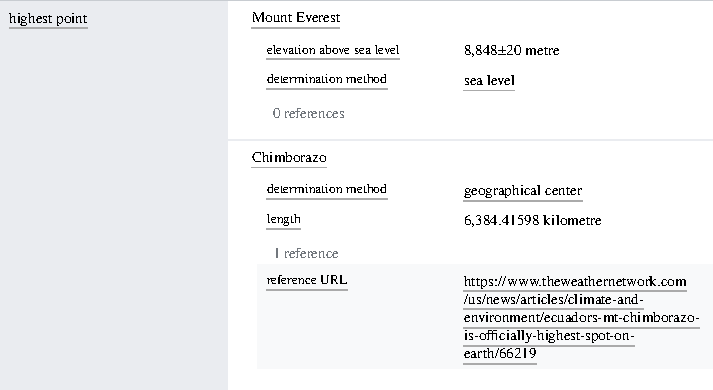
\includegraphics[width=\linewidth]{pics/example-statement}
  \caption{Zwei Statements des Items "`Erde"' für die Property "`höchster Punkt"'}
  \label{fig:sample-statement}
\end{figure} 

Eine bereits existierende Möglichkeit zur Abfrage von Daten ist der Wikidata Query Service \cite{wd-sparql}. 
Mit diesem Service lassen sich komplexe Abfragen auf den Daten von Wikidata beantworten.
Allerdings ist es mit diesem Service sehr schwierig, die kompletten Daten zu einem Thema abzurufen, da das Schema des Query Services die Daten sehr stark zerlegt.
Außerdem ist die Laufzeit von Abfragen auf eine Minute limitiert, was bei großen Datenmengen ein Problem ist.
Das dieses Limit nicht nur ein theoretisches Problem ist, zeigt eine Arbeit zur Verwendung von Referenzen in Wikidata\cite{wd-wk-common-references}.
Die Autoren mussten die Abfrage nach allen Referenzen von einem Mitarbeiter von Wikimedia Deutschland ausführen lassen, da sie nicht innherhalb des Limits terminiert.

Das in dieser Arbeit vorgestellte System füllt die Nische zwischen dem vollständigen Export und dem Wikidata Query Service.
Durch die Angabe von Filtern wird eine Teilmenge der Daten definiert.
Aus den Daten, die diese Filter erfüllen, wird dann ein individualisierter Datenexport (Dump) generiert.
Über eine Integration mit dem Archivierungsdienst Zenodo\footnote{\url{https://zenodo.org/}} können die generierten Dumps direkt archiviert werden.
Zenodo generiert einen Digital Object Identifier (DOI), sodass die Dumps danach einfach in wissenschaftlichen Veröffentlichungen zitiert werden können.

\section{Struktur der Arbeit}
Im zweiten Kapitel wird zunächst notwendiges Hintergrundwissen zum Aufbau von Wikidata und den verwendeten Technologien vermittelt.
Danach werden in \cref{chap:requirements} die Anforderung an das System detaillierter beschrieben und verwandte Arbeiten verglichen.
In \cref{chap:design} wird dann das Design des Systems erarbeitet, dessen Implementierung in \cref{chap:implementation} vorgestellt wird.
Die Evaluation der Implementierung auf Korrektheit und Vollständigkeit erfolgt in \cref{chap:evaluation}, mit einem  Vergleich zwischen den existierenden Wikidata-Dumps und den generierten Dumps.
Im \cref{chap:conclusion} wird schließlich ein Ausblick auf mögliche Verbesserungen gegeben und eine Zusammenfassung des Ergebnis präsentiert.

Dabei werden die folgenden Beiträge geleistet:
\begin{itemize}
  \item Analyse verschiedener Systemdesigns zur Generierung angepasster Wikidata-Dumps
  \item Entwurf einer Spezifikation für Filterkriterien
  \item Implementierung des vorgestellten Designs mit Wikidata Toolkit\footnote{https://github.com/Wikidata/Wikidata-Toolkit}. Wikidata-Toolkit ist eine Bibliothek zum Verarbeiten und Erzeugen von Wikidata Dumps.
  \item Evaluation der Vollständigkeit und Korrektheit des RDF-Exports von Wikidata Toolkit
\end{itemize}